\section{Интервальные версии: более широкие запрещённые отрезки}
\label{sec:wide}

Метод даёт не только оценки на $\chi(\R^n)$, но и раскраски, запрещающие целый
отрезок расстояний. Здесь собраны такие результаты: компромисс
<<цвета\,$\leftrightarrow$\,ширина>> в $\R^4$, лестницы ширин в $\R^2$--$\R^6$ и
улучшения в $\R^3$.

\subsection{Более широкий интервал в $\R^4$: $\chi(\R^4,[1,\ell])\le48$}


При индексе~$48$ та же оптимизация даёт заметно большую ширину. Для рациональной
решётки с матрицей Грама
\[
Q_{48}=\begin{pmatrix}
\tfrac{137}{12}&\tfrac{13}{7}&-\tfrac{61}{10}&-\tfrac{18}{5}\\[2pt]
\tfrac{13}{7}&7&-\tfrac{25}{9}&-\tfrac{37}{12}\\[2pt]
-\tfrac{61}{10}&-\tfrac{25}{9}&12&-\tfrac{17}{11}\\[2pt]
-\tfrac{18}{5}&-\tfrac{37}{12}&-\tfrac{17}{11}&\tfrac{44}{5}
\end{pmatrix}
\]
и подрешётки индекса~$48$ с наддиагональю $(28,16,30)$ в последнем столбце
получается $d=1{,}039657677\ldots$ (здесь $\lambda_1^2=7$,
$\diam^2P=19{,}141641$, $D^2\ge20{,}689971$); тем же точным сертификатом
доказывается
\[
\chi\bigl(\R^4,[1,\ell]\bigr)\le48\qquad(\ell\le1{,}0396).
\]
Численный оптимум при индексе~$48$ достигает $d=1{,}0432696$. Итак, увеличив
число цветов на три ($45\to48$), можно заметно расширить запрещённый интервал
($1{,}015\to1{,}0396$) --- этот компромисс <<цвета${}\leftrightarrow{}$ширина>>
ранее не отмечался.

\subsection{Сводка результатов в $\R^4$}

Таблица~\ref{tab:r4} собирает все три полученные решёточные раскраски $\R^4$:
рекордную по числу цветов ($45$) и две с более широким запрещённым интервалом
($46$, $48$). Каждая задаётся рациональной решёткой общего положения (ячейка
Вороного имеет $f$-вектор $(120,240,150,30)$ --- такой же, как у четырёхмерного
пермутоэдра) и подрешёткой с циклической
матрицей перехода; для каждой доказан точный сертификат $d>\ell_0$. Матрицы
Грама для $k=45$ и $k=48$ выписаны выше, для $k=46$ --- в файле
\path{audit-data/results/cert46.json}.

\begin{table}[h]
\centering
\caption{Полученные раскраски $\R^4$: $\chi(\R^4,[1,\ell])\le k$ при
$\ell\le\ell_0$. Столбец <<знам.>> --- наибольший знаменатель рациональной
матрицы Грама; <<$d$ (числ.)>> --- ширина численного оптимума; десятичные
значения <<$d$ (рацион.)>> округлены вниз.}
\label{tab:r4}
\small
\begin{tabular}{c c c c c l}
\toprule
$k$ & $\ell_0$ (сертиф.) & $d$ (рацион.) & $d$ (числ.) & знам. & примечание\\
\midrule
\textbf{45} & $\mathbf{1{,}015}$ & $1{,}016339$ & $1{,}017401$ & $16$
  & \textbf{рекорд по числу цветов}\\
46 & $1{,}004$ & $1{,}005068$ & $1{,}005405$ & $24$ & промежуточный\\
48 & $1{,}0396$ & $1{,}039657$ & $1{,}043270$ & $12$ & наибольший интервал\\
\bottomrule
\end{tabular}
\end{table}

\subsection{Лестницы ширин и улучшения в $\R^3$}\label{sec:stair}

Дешевизна оценки формы (\S\ref{sec:big}) позволяет строить \emph{лестницы ширин}
и в старших размерностях: при большем числе
цветов запрещённый интервал расширяется (на фиксированной $A_5^*$ до
$[1,\,1{,}265]$ при $k=300$, табл.~\ref{tab:stair56}). При $n\ge7$ запрещённое множество быстро растёт
($|F_1|\approx1{,}9\cdot10^4$ для $A_7^*$,
${\approx}3{,}5\cdot10^4$ для $E_7$), поэтому сплошной перебор индексов
становится дорогим и поиск ведётся по \emph{курируемым} индексам.


Рис.~\ref{fig:stair} показывает <<лестницы>> максимальной ширины $d(k)$ ---
бегущий максимум по классическим решёткам --- для $\R^2$, $\R^3$, $\R^4$. Порог
$d=1$ впервые достигается при $k=7$ (шестиугольная решётка, $\R^2$), $k=15$
(BCC, $\R^3$) и $k=49$ по классическим решёткам в $\R^4$ (решётки общего
положения опускают его до~$45$, \S\ref{sec:main}).

\begin{figure}[t]
\centering
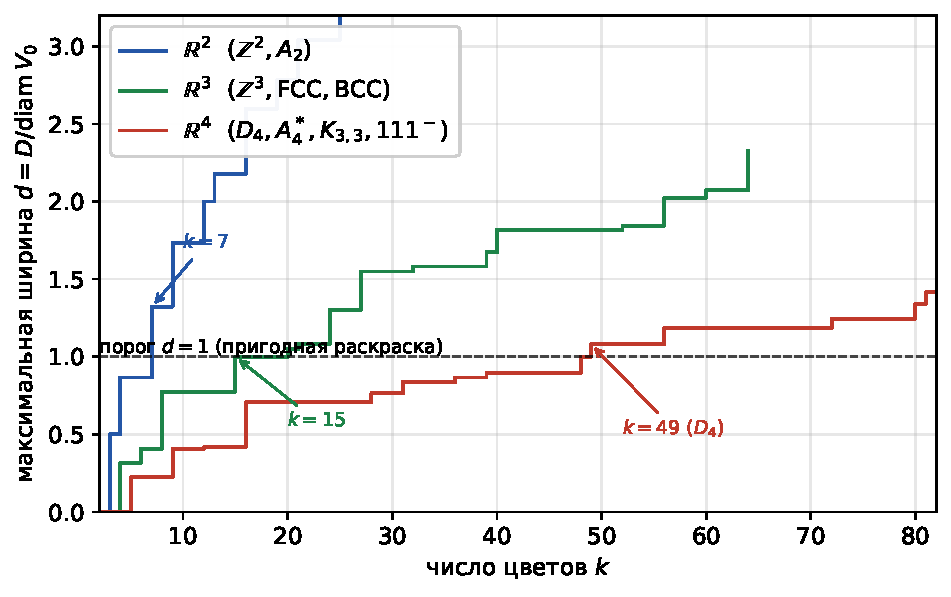
\includegraphics[width=0.74\textwidth]{fig_staircase.pdf}
\caption{Максимальная нормированная ширина $d(k)$ как функция числа цветов $k$
для $\R^2$, $\R^3$, $\R^4$ (бегущий максимум по классическим решёткам каждой
размерности). Пунктир --- порог $d=1$: правее точки пересечения раскраска в $k$
цветов правильна для классического расстояния.}
\label{fig:stair}
\end{figure}

(Здесь запись <<$\R^4$, $k=49$>> относится к классическим решёткам; выход в
решётки общего положения даёт $46$, $48$ и рекордные $45$ цветов, \S\ref{sec:main}.)

\paragraph{Размерность 3: оптимальность 15 цветов и расширение интервала.}
В отличие от $\R^4$, в $\R^3$ число цветов уменьшить нельзя: нижняя граница
Кулсона для решёточных раскрасок $\chi_s\ge2^{n+1}-1$ \cite{Coulson,ABPR} даёт
$\chi_s(\R^3)\ge15$, и это подтверждается численно --- оптимизация метрики при
$k=8,\dots,14$ ни разу не достигает порога $d=1$ (максимум $d=0{,}900$ при
$k=14$). Значит, $15$ цветов --- оптимум среди решёточных раскрасок $\R^3$.

Исторически первая решёточная $15$-раскраска предложена Кулсоном
\cite{Coulson} на ОЦК-решётке. Рассмотрим её внутри однопараметрического
семейства форм
\[
G(\alpha)=\begin{pmatrix}1&-\alpha&2\alpha-1\\-\alpha&1&-\alpha\\
2\alpha-1&-\alpha&1\end{pmatrix},
\qquad
T=\begin{pmatrix}1&0&11\\0&1&7\\0&0&15\end{pmatrix},
\]
где матрица перехода $T$ подрешётки индекса~$15$ \emph{фиксирована}, а при
$\alpha=1/3$ форма пропорциональна ОЦК --- это случай Кулсона. Решение
KKT-систем связывающих орбит в замкнутой форме даёт
\[
D^2_{(3,2,2)}=\frac{4\alpha^2+3\alpha+1}{\alpha+1},\qquad
D^2_{(2,1,-1)}=\frac{2(5\alpha^2-6\alpha+2)}{1-\alpha},\qquad
\diam^2 V_0=2-\alpha,
\]
откуда при $\alpha=1/3$ ширина равна \emph{ровно} $1$ (проверено и полным
точным аудитом: $12$ векторов окна, все KKT-сертификаты): интервал вырожден,
и предложение~\ref{prop:crit}, требующее строгого $\ell<d$, к случаю Кулсона
неприменимо --- его оценка $\chi(\R^3)\le15$ получена отдельным разбором
границ ячеек \cite{Coulson}. Но уже малая деформация даёт строгий запас:
максимум семейства достигается в корне кубики
$14\alpha^3-3\alpha^2-10\alpha+3=0$, то есть при
$\alpha^*=0{,}3136953\ldots$, со значением $d^*=1{,}0265986\ldots$; лучший
найденный численный оптимум по всем шестипараметрическим формам
($1{,}0265930$) его не превосходит, так что семейство $G(\alpha)$,
по-видимому, содержит глобальный оптимум $k=15$. В рациональной точке
$\alpha=16/51$ (целочисленный грамиан $51\,G$) вся цепочка проверена в точной
арифметике дробей: $d^2=1586/1505$, и
\[
\chi\bigl(\R^3,[1,\ell]\bigr)\le15\qquad(\ell\le513/500=1{,}026)
\]
--- статус \textbf{[С]}: целый запрещённый интервал вместо единственного
расстояния у Кулсона. Сертификат --- обе точки семейства, включая
калибровочную $\alpha=1/3$, ---
\path{audit-data/results/dim3_k15_certificate.json}.

При $k>15$ оптимизация метрики по всему пространству форм заметно улучшает
нашу прежнюю таблицу \cite{Ivanov2011} для $\R^3$ (табл.~\ref{tab:r3}; каждое значение
--- явная решётка и подрешётка): при $k=21,23,24$ ширины существенно больше, а
для многих $k$ (в т.ч. для порогового $k=15$) оценки получены впервые.

\begin{table}[h]
\centering
\caption{Ширина $d$ запрещённого интервала для $\chi(\R^3,[1,\ell])\le k$ при
оптимизации метрики по всему пространству квадратичных форм (выборка $k$).
Прочерк --- значение, отсутствующее в \cite{Ivanov2011}.}
\label{tab:r3}
\small
\begin{tabular}{c cccccccccc}
\toprule
$k$ & 15 & 18 & 20 & 21 & 23 & 24 & 27 & 32 & 40 & 49\\
\midrule
$d$ (наст. раб.) & $\mathbf{1{,}026}$ & $1{,}116$ & $1{,}172$ & $\mathbf{1{,}263}$
  & $\mathbf{1{,}253}$ & $\mathbf{1{,}364}$ & $1{,}549$ & $1{,}581$ & $1{,}822$
  & $1{,}914$\\
$d$ (\cite{Ivanov2011}) & --- & $1{,}116$ & --- & $1{,}134$ & $1{,}137$ &
  $1{,}304$ & $1{,}549$ & --- & --- & ---\\
\bottomrule
\end{tabular}
\end{table}

\noindent Попутно исправлены три опечатки, допущенные в матрицах подрешёток
в~\cite{Ivanov2011}. Верные матрицы таковы: для $\R^3$ при $k=21$ ---
диагональ $(3,1,7)$ с наддиагональю $(0,0,5)$; для разрежённой серии при $k=14$
--- наддиагонали $(0,0,12)$ и $(0,0,10)$.

\paragraph{Размерности 5 и 6: лестницы на $A_5^*$ и $E_6^*$.} Дешёвая оценка
формы (\S\ref{sec:big}) впервые позволяет проследить лестницу ширин и в старших
размерностях. Для $\R^5$ подрешётки решётки $A_5^*$ различных индексов дают
расширяющийся запрещённый интервал (табл.~\ref{tab:stair56}): порог $d=1$
на \emph{фиксированной} $A_5^*$ достигается при $k=140$ (конструкция $C_5$,
$d=\sqrt{39/35}$), а уже при
$k=196,270,300$ ширина растёт до $\sqrt{7/5},\ \sqrt{54/35},\ \sqrt{8/5}$ ---
интервальные оценки $\chi(\R^5,[1,\ell])\le k$, ранее не отмечавшиеся. В $\R^6$
метод воспроизводит эйзенштейнову подрешётку $E_6^*/343$ с точной шириной
$\sqrt{7/6}$ (\S\ref{sec:extra}) как \emph{минимальный} по числу цветов
решёточный порог. Раскраски найдены масштабируемым поиском
(\S\ref{sec:big}); нормированные ширины вычислены как $\min_{v\in\Gamma\setminus0}
D(v)/\diam V_0$ и совпадают с указанными рациональными $d^2$ до $5$ знаков.

\begin{table}[h]
\centering
\caption{Лестница ширин запрещённого интервала в $\R^5$ (решётка $A_5^*$) и
опорная точка в $\R^6$ (решётка $E_6^*$): $\chi(\R^n,[1,\ell])\le k$ при
$\ell<d$. Строка $k=140$ совпадает с точным результатом АБПР (табл. в~\S\ref{sec:extra}); новая конструкция индекса~$132$ использует другую форму и
приведена в теореме~\ref{thm:r5}.}
\label{tab:stair56}
\small
\begin{tabular}{c c l l l}
\toprule
$n$ & $k$ & решётка & $d^2$ & $d$\\
\midrule
5 & 140 & $A_5^*$ & $39/35$ & $1{,}0556$\\
5 & 196 & $A_5^*$ & $7/5$   & $1{,}1832$\\
5 & 270 & $A_5^*$ & $54/35$ & $1{,}2421$\\
5 & 300 & $A_5^*$ & $8/5$   & $1{,}2649$\\
6 & 343 & $(3+\omega)E_6^*$ & $7/6$ & $1{,}0801$\\
\bottomrule
\end{tabular}
\end{table}


